Med udgangspunkt i øvelsesopgave~\ref{sierpinski.ov} skal du i denne opgave implementere en GUI-applikation der kan tegne en version af X-fractalen som illustreret nedenfor (eventuelt i en dybde større end 2).
\begin{center}
  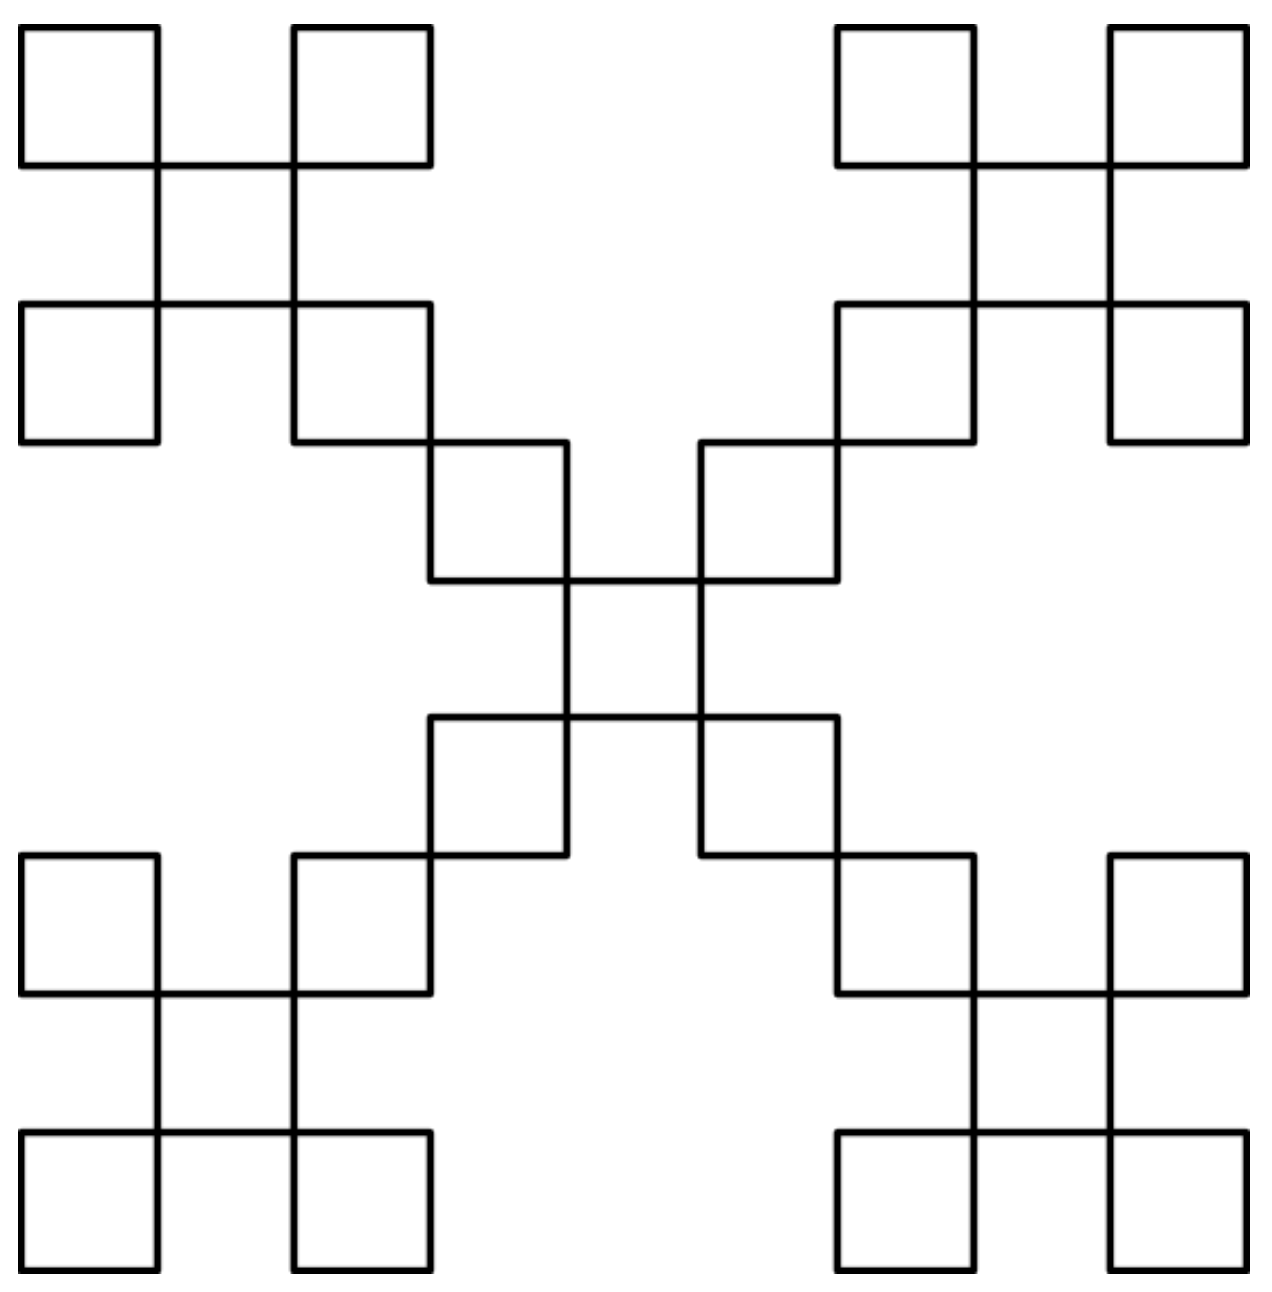
\includegraphics[width=0.3\textwidth]{xfractal.png}
\end{center}
Bemærk at det ikke er et krav at dybden på fraktalen skal kunne styres med piletasterne som det er tilfældet med Sierpinski-fraktalen i øvelsesopgave~\ref{sierpinskikeys.ov}.

